\section{Methods}
\begin{figure*}[t]
    \centering
    % 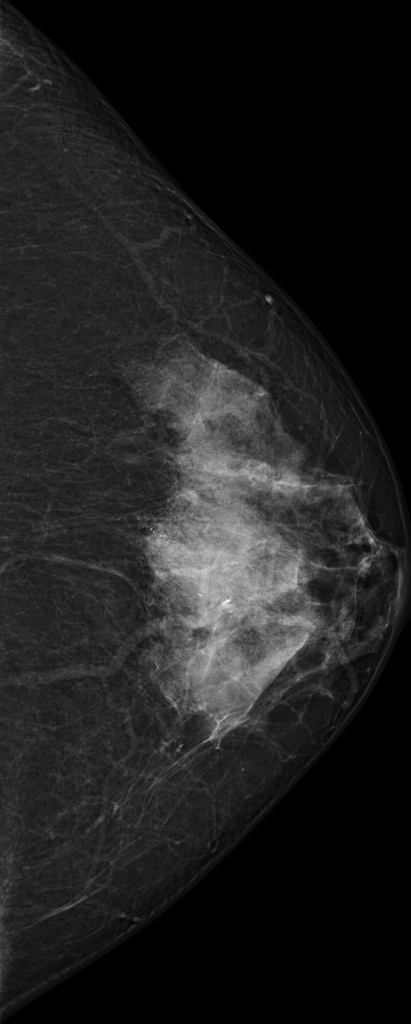
\includegraphics[scale = 0.4]{Final/Figures/Correctly_classify.png}
    % \caption{Well-Predicted Image Sample in classification}
    % \label{fig: classified_True}
    % 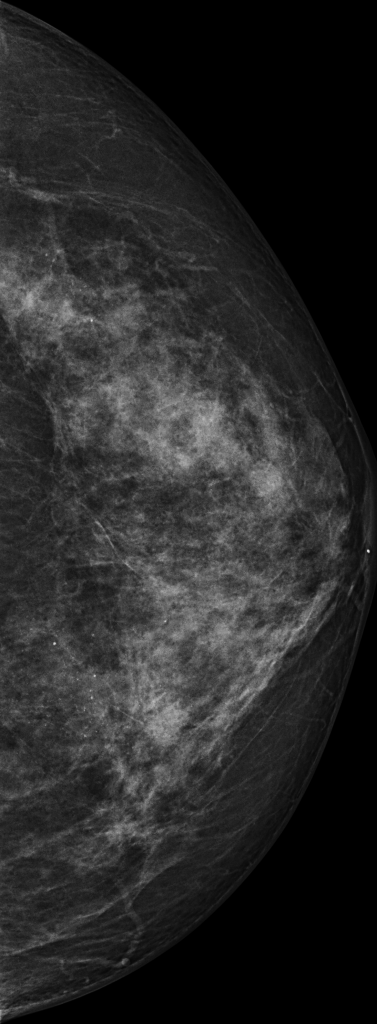
\includegraphics[scale = 0.4]{Final/Figures/Incorrectly_classify.png}
    % \caption{Poorly-Predicted Image Sample in classification}
    % \label{fig: classified_False}
    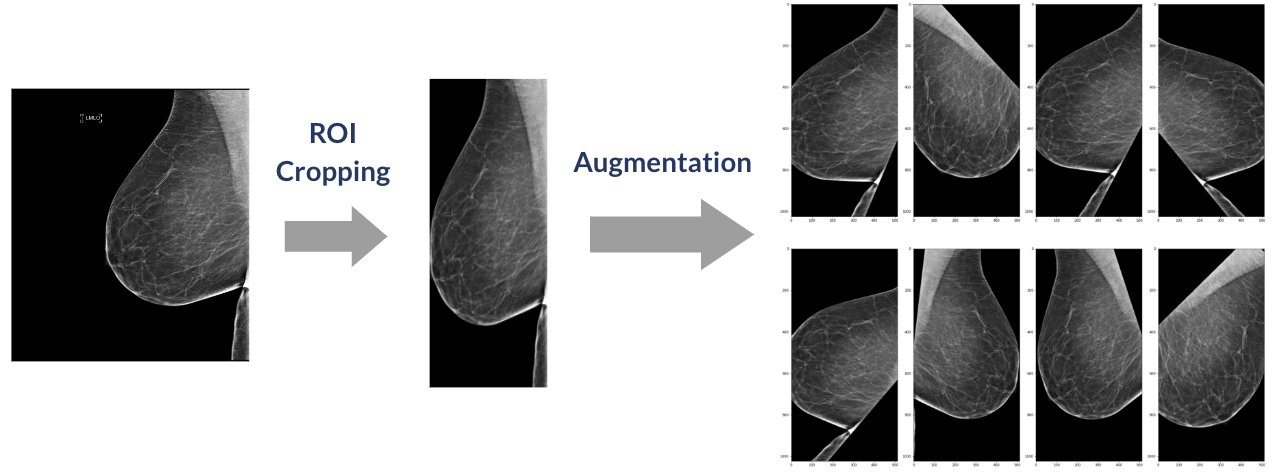
\includegraphics[scale = 0.7]{Final/Figures/image_preprocess.png}
    \caption{ROI Cropped and Augmented Image Sample}
\end{figure*}

This section presents our model architecture, comprising six key components: ROI Crop, Image Augmentation, Backbone ML model, Weighted Loss, Threshold, and Auxiliary Prediction. As depicted in Figure 2 model flow-diagram, our preprocessing pipeline initially employs ROI Crop and Augmentation techniques to enhance each breast cancer image before feeding it into the Backbone model. We experimented with both CNN and ViT pre-trained models as our Backbone model. However, we encountered a challenge in finding a suitable CNN and ViT pre-trained model on medical images. Therefore, we resorted to using general pre-trained CNN and ViT models (on ImageNet) as done by most other researchers in the field${}^{[5][6]}$. 

To address the issue of data imbalance during the training of our ML model, we employed a weighted loss function. To determine the best threshold for distinguishing cancer images, we used a 5-fold cross-validation approach. Finally, we evaluated our model's performance using test data.

\subsection{ROI Cropping}
% \begin{figure}[H]
%     \centering
%     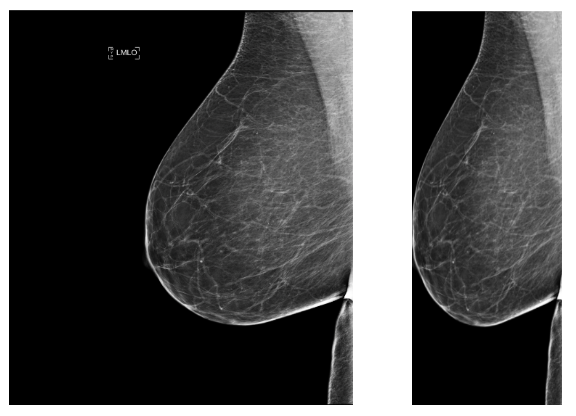
\includegraphics[scale = 0.6]{Final/Figures/original+roi_cropped.png}
%     \caption{Original Image (left) and ROI Cropped Image (right)}
%     \label{fig:sample img for roi crop}
% \end{figure}
ROI(Region of Interest) cropping is a computer vision technique that extracts an image's specific object or area of interest by defining a rectangular region and cropping and resizing the image to include only the relevant pixels. This method is particularly useful when the object is small relative to the overall image or when background noise or clutter can interfere with detection. In our analysis, we employed ROI cropping to extract the breast area and exclude other non-breast regions from the images.

\subsection{Augmentation}
After ROI cropping, we performed image augmentation to increase the diversity and robustness of the dataset by applying multiple transformations. Image augmentation is a computer vision technique that artificially expands the dataset by applying various transformations to the original images. Our analysis employed several transformations, including horizontal flip, rotation, auto contrast, resize crop, Gaussian blur, and shift to increase diversity. Additionally, we reduced noise and improved the model's resilience to small variations in input data by using Gaussian blur. Furthermore, we utilized auto contrast to enhance image contrast, highlighting more details and facilitating cancer detection.
% \begin{figure}[H]
%     \centering
%     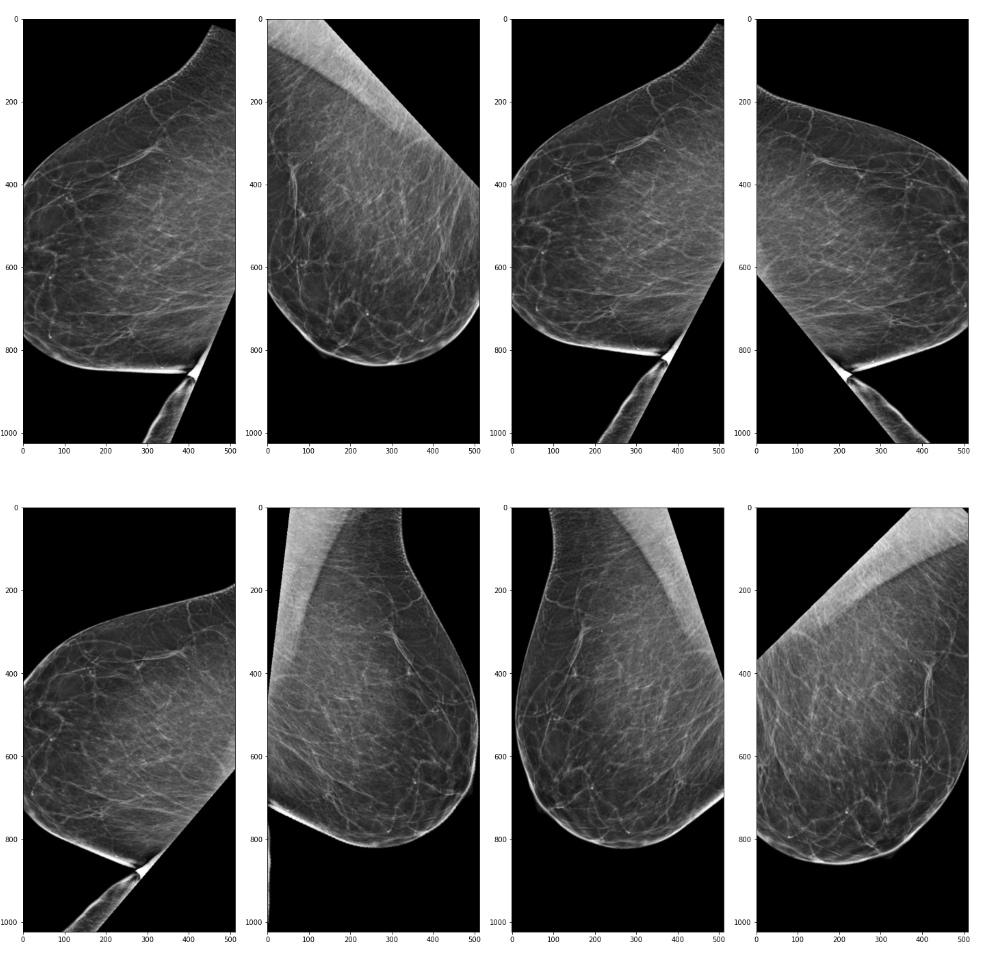
\includegraphics[scale = 0.4]{Final/Figures/augmented.png}
%     \caption{Augmented Image Sample after ROI cropping}
%     \label{fig: sample img for aug}
% \end{figure}

\subsection{Backbone Model}
For our study, we focused majorly on CNN models. We found much research that reported usage of ResNet (Residual Networks) CNN architecture and it's variants. It is a popular CNN architecture that introduced the concept of residual learning to address the vanishing gradient problem in deep networks. It utilizes skip connections to allow the gradients to flow directly through the network, enabling the training of very deep networks. Furthermore, a ResNeXt is a convolutional neural network architecture that builds on the ResNet architecture by introducing a new 'cardinality' element.  It repeats a building block that aggregates a set of transformations with the same topology, thus capturing more diverse features. We saw our best results using a variant of ResNext, called SE ResNeXt. 

Furthermore, we also used state-of-the-art architecture in the form of a Vision Transformer (ViT). By replacing conventional convolutional layers with self-attention layers, a Vit architecture is reported to enable the network to process image patches in a more flexible and efficient manner. For our study, we used pre-trained models in the family of DeiT family of ViT models. The base architecture consists of a stack of transformer blocks, with each block having self-attention and feedforward layers.

\subsubsection{Weighted Loss}
As we explained in the \textit{Section 4: Data}, we choose a highly imbalanced dataset that is more likely to be found in reality. To solve this imbalance, we use the weighted loss function, one of the most well-known techniques to tackle a problem in imbalanced data, giving more weight to the loss of cancer images. We employed weighted loss rather than weighted sampling since it performed better empirically.

\subsubsection{Threshold}
For setting the threshold, we used the sigmoid function since there are only two classes in the dataset (malignant and benign) in order to improve the model performance by discriminating between malignant (cancer) and benign (non-cancer) images in evaluation and testing. The best threshold was determined by evaluation data and results, and then it was employed in the testing set.
 
\subsubsection{Auxiliary Prediction}
In addition to the techniques described in Sections 4.4 and 4.5, we have incorporated auxiliary loss predictions into our model by adding extra output branches to the network that predict intermediate outcomes related to the main task of classifying mammogram images. Our approach uses 11 additional features (listed in Table 2) as intermediate predictions to compute additional loss, which is then combined with the main loss function to optimize the model during training. Incorporating auxiliary loss predictions has been shown to help improve model performance by reducing the risk of gradient vanishing, promoting the learning of diverse features, preventing overfitting, and providing regularization to the network. ${}^{[9]}$

\subsection{Experiment}
In this section, we explain our experiment settings and evaluation metrics. Also, we illustrate our baseline and follow-up models in which our major components are added to a baseline model.

\subsection{Experiment Settings and Evaluation Metrics} 
We utilize 5-fold cross-validation to evaluate all models with our training dataset. Original images are high-resolution dcm(dicom) format files, so we converted dcm files to png files. Also, to reduce the training and test overhead and fit a pre-trained backbone model, we resized images to smaller sizes. About the model parameters, first, we adopt other competitors’ parameters and change them little by little to get a better result. We finetune our model for 3-10 epochs(depending on the backbone model). The batch size is 16, and the learning rate is 0.0002 to 0.0008. For backbone models we tried both freezing(transfer learning) and no freezing, but all models we tested made better results without freezing.

\subsection{Baseline and Implemented Model Description}
% We set our baseline is just applying a backbone model on resized original images (none of ROI crop, augmentation or others) with weighted loss. We tested two backbone models. One is CNN named 'seresnext50\_32x4d' and the other is ViT named 'deit3\_base\_patch16\_384'. We tried other models such as eva02, swin-ViT, google/vit, but the above models made better performance. After we found out CNN makes better results on average, we added components one by one to our backbone model. Also, most kaggle participants and almost all top rankers use CNN.

% First, we added an ROI crop to get more useful images. Original images have large useless black pixel area, so we found ROI cropped images from kaggle site and used it. This is our second model.

% Next, we added threshold technique. We realized that if we use threshold values which discriminate against cancer images other than 0.5, validation f1 score improves. Also, sometimes(not always) it also lead to better test result, too. We calculate the f1 score varying threshold value from 0 to 1 by 0.01, and choose the best threshold value that makes the best f1 score of that CV fold. We choose the best fold model with threshold value and apply it to test data. This is our third model.

% Third, we add image augmentation components. Because all images are ROI cropped x-ray images of breasts, we assume that a big change in image is not useful. Therefore, we apply little changes such as rotate a little, resize a little bit and crop. This is our fourth model.

% Finally, we adopt Auxiliary Prediction. Before adding this component, our model only predicts cancer or not and also loss is only dependent on cancer because our goal is predicting cancer images. However, our model predicts other features in kaggle data. There are 11 features that can predict which is 'site\_id', 'laterality', 'view', 'implant', 'biopsy', 'invasive', 'BIRADS', 'density', 'difficult\_negative\_case', 'machine\_id', 'age'. Our model predicts these 11 features and calculates loss. This loss is also used during backpropagation. This is our fifth and final model.

For the baseline model, we applied only a backbone model on resized original images with a weighted loss function. Specifically, we employed two backbone models, the 'seresnext50\_32x4d' CNN and the 'deit3\_base\_patch16\_384' ViT. While we evaluated several other models, including eva02, swin-ViT, and google/vit, our chosen backbone models demonstrated superior performance. Given that CNN models were prevalent among top Kaggle participants, we opted to focus on this type of model. 

To improve performance, we gradually introduced several additional components to our baseline model. Firstly, we incorporated an ROI crop module to eliminate useless black pixel areas in the original images. We obtained ROI-cropped images from Kaggle's public dataset and applied them as the basis for our second model. 

Secondly, we introduced thresholding techniques to identify cancer images with improved accuracy. By varying the threshold value from 0 to 1 in increments of 0.01, we computed the F1 score and selected the best threshold value that resulted in the highest F1 score. We applied this approach to both validation and test datasets, resulting in our third model. 
%%%%%%%%%%%%%%%%%%%%%%%%%%%%%%%%%%%%%%%%%%%%%%%%%%%%%%%%%%%%%%%%%%
%%%%% RESULT TABLE %%%%%
\begin{table*}[t]
\centering
%\resizebox{\columnwidth}{!}{
%\footnotesize
\begin{tabular}{|c|c|c|c|c|c|c|}
    \hline
\multicolumn{2}{|c|}{ } & Evaluation &  \multicolumn{4}{c|}{Test} \\
\hline
Setting & Model & F1 & F1 & Recall & Precision & Accuracy \\
\hline\hline
\multirow{2}{*}{Resized Original} & CNN(ResNeXt) & 0.047 & 0.027 & 0.022 & 0.035 & 0.966 \\
& ViT(deit3) & 0.037 & 0.0 & 0.0 & 0.0 & 0.979 \\
\hline
+ ROI Crop & CNN & 0.057 & 0.108 & 0.359 & 0.063 & 0.874\\
\hline
+ Threshold & CNN & 0.122 & 0.076 & 0.351 & 0.043 & 0.820 \\
\hline
+ Augmentation & CNN & 0.161 & 0.044 & 0.043 & 0.043 & 0.959\\
\hline
\multirow{2}{*}{+ Auxiliary Prediction} & CNN(ResNeXt) & 0.345 &  0.314 & 0.290 & 0.342 & 0.973 \\
& ViT(deit3) & 0.130 & 0.063 & 0.126 & 0.042 & 0.921 \\
\hline
\end{tabular}%}
\caption{Results of Models Implementation}
\end{table*}
%%%%%%%%%%%%%%%%%%%%%%%%%%%%%%%%%%%%%%%%%%%%%%%%%%%%%%%%%%%%%%%%%%
Next, we introduced image augmentation to the ROI-cropped X-ray images of breasts. As we assumed that large image changes were not useful, we applied minor alterations such as slight rotation, resizing, and cropping. This resulted in our fourth model. 

Finally, we incorporated an auxiliary prediction module to predict features beyond cancer/non-cancer. Specifically, we trained our model to predict 11 additional features, including site\_id, laterality, view, implant, biopsy, invasive, BIRADS, density, difficult\_negative\_case, machine\_id, and age. This module enabled our model to capture more information and improve overall performance.
